% L14a paper trading with an AI assistant. Top: a laptop running the AI assistant (Claude
% Code) sends a tool call to the MCP server, a rack whose units are three of its tools;
% the server holds the key and secret and sends an API request to the Alpaca paper account,
% which fills each order against the latest quotes (IEX). Gray arrows carry the result and
% the order status back.
%
% November 19, 2026: drawn in the style of the L13a schematics (schematic-style.tex).
% Checks: the tool names match src/Catalog.jl of alpaca-mcp.
% November 23, 2026: the bottom panel (the life of an order) removed, with its lecture text.
\documentclass[tikz,border=6pt]{standalone}
% Shared style for the L14a schematics (November 19, 2026), \input by each Fig-L14a-*.tex.
% Copied from week-13/L13a/figs/jumphmm-diagram.tex (the week-12 schematic style): same fonts,
% ink, accent colors, boxes, and arrows, plus a monospace font for tool names and order
% statuses. The notebook SVG carries a dark palette added by theme_svg.py; every color here
% must be mapped there.
\usepackage[no-math]{fontspec}
\IfFontExistsTF{Arial}{\setsansfont{Arial}}{\setsansfont{TeX Gyre Heros}}
\renewcommand{\familydefault}{\sfdefault}
\IfFontExistsTF{Menlo}{\setmonofont[Scale=0.92]{Menlo}}{}
\usepackage{amsmath,amssymb}
\usetikzlibrary{arrows.meta,calc,positioning,decorations.pathreplacing}

\definecolor{vnink}{HTML}{202124}
\definecolor{gdblue}{HTML}{0091FF}
\definecolor{gdred}{HTML}{E02020}
\definecolor{gdgray}{HTML}{6D7278}
\definecolor{saorange}{HTML}{F08C00}
\definecolor{boxfill}{HTML}{F1F3F4}
\definecolor{orangefill}{HTML}{FFE8C7}
\definecolor{bluefill}{HTML}{E5F3FF}
\definecolor{redfill}{HTML}{FDE8E8}
\definecolor{gridgray}{HTML}{E3E5E8}

\tikzset{
  every picture/.append style={x=1cm, y=1cm, font=\sffamily\small, text=vnink},
  % boxes and arrows, as in the L12a schematics
  flow/.style={draw=vnink, line width=0.9pt, -{Latex[length=2.4mm, width=1.7mm]}},
  feedback/.style={draw=saorange, line width=1.2pt, -{Latex[length=2.6mm, width=1.9mm]}, rounded corners=6pt},
  sumbox/.style={draw=vnink, fill=boxfill, line width=0.8pt, rounded corners=3pt, inner sep=5pt, align=center},
  note/.style={text=gdgray, font=\sffamily\footnotesize, align=center},
  state/.style={circle, draw=vnink, fill=white, line width=1.0pt, minimum size=1.1cm, inner sep=0pt, font=\sffamily\normalsize},
  % plots, as in the L10b profit diagrams
  axis/.style={draw=vnink, line width=0.8pt, -{Latex[length=2.6mm, width=1.8mm]}},
  spine/.style={draw=vnink, line width=0.8pt},
  curve/.style={draw=vnink, line width=1.6pt, line join=round, line cap=round},
  series/.style={draw=gdgray, line width=0.9pt, line join=round},
  drop/.style={draw=gdgray, line width=0.8pt, dash pattern=on 3pt off 2pt},
  pt/.style={circle, draw=vnink, fill=white, line width=1.0pt, inner sep=0pt, minimum size=2.0mm},
}


\begin{document}
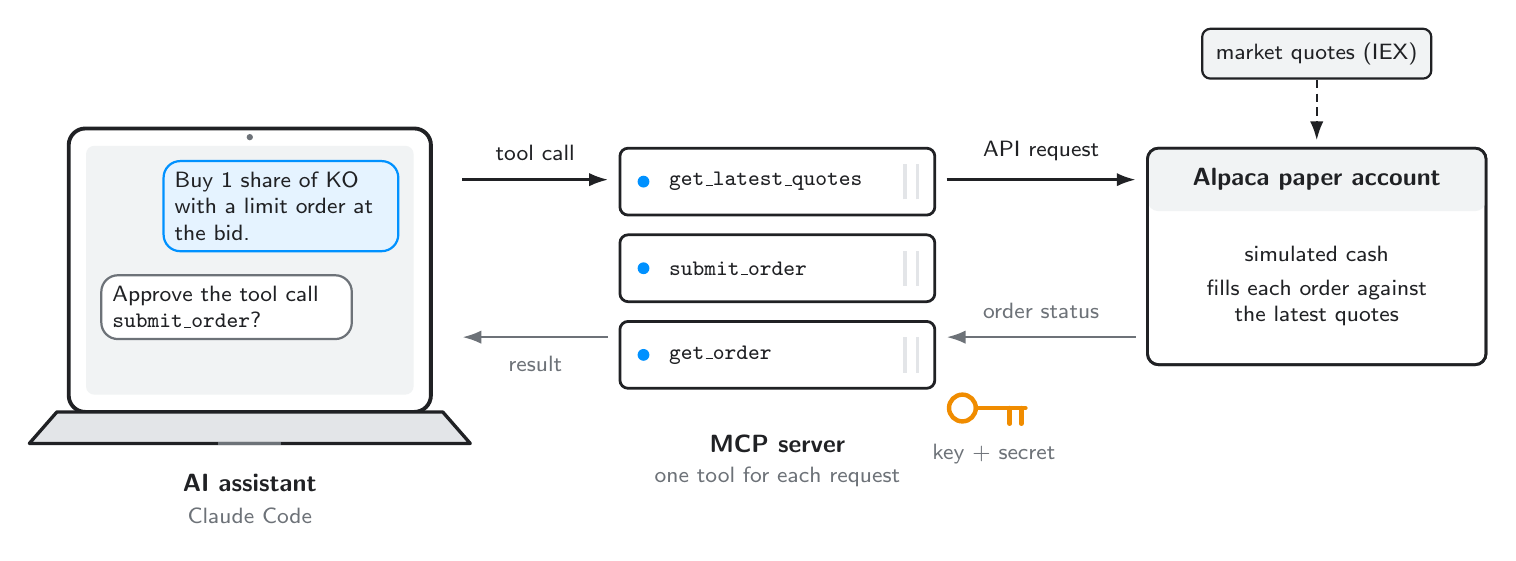
\begin{tikzpicture}[
  unit/.style={draw=vnink, fill=white, line width=1.0pt, rounded corners=3pt},
  bubble/.style={rounded corners=6pt, line width=0.8pt, font=\sffamily\footnotesize, align=left, inner sep=4pt},
  back/.style={draw=gdgray, line width=0.9pt, -{Latex[length=2.4mm, width=1.7mm]}},
  label/.style={font=\sffamily\small\bfseries, align=center},
]
  % ---------------------------------------------------------------- the AI assistant
  % the laptop: bezel, screen, camera, and keyboard base
  \draw[draw=vnink, fill=white, line width=1.4pt, rounded corners=6pt] (0.0, 3.0) rectangle (4.6, 6.6);
  \fill[boxfill, rounded corners=3pt] (0.22, 3.22) rectangle (4.38, 6.38);
  \fill[gdgray] (2.3, 6.49) circle (0.04);
  \draw[draw=vnink, fill=gridgray, line width=1.2pt, line join=round]
    (-0.15, 3.0) -- (4.75, 3.0) -- (5.1, 2.6) -- (-0.5, 2.6) -- cycle;
  \draw[draw=gdgray, line width=0.8pt] (1.9, 2.6) -- (2.7, 2.6);

  % the chat on the screen: our request, and the assistant asking for approval
  \node[bubble, draw=gdblue, fill=bluefill, anchor=north east, text width=2.7cm] (ask) at (4.2, 6.2)
    {Buy 1 share of KO with a limit order at the bid.};
  \node[bubble, draw=gdgray, fill=white, anchor=north west, text width=2.9cm] (reply) at (0.4, 4.75)
    {Approve the tool call \texttt{submit\_order}?};
  \node[label] at (2.3, 2.1) {AI assistant};
  \node[note] at (2.3, 1.68) {Claude Code};

  % ---------------------------------------------------------------- the MCP server
  % a rack of three units, each one tool, with a status light and vents
  \foreach \y/\tool in {5.5/get\_latest\_quotes, 4.4/submit\_order, 3.3/get\_order} {
    \draw[unit] (7.0, \y) rectangle (11.0, \y + 0.85);
    \fill[gdblue] (7.3, \y + 0.425) circle (0.075);
    \node[anchor=west, font=\ttfamily\footnotesize] at (7.5, \y + 0.425) {\tool};
    \draw[draw=gridgray, line width=1.2pt] (10.62, \y + 0.2) -- (10.62, \y + 0.65);
    \draw[draw=gridgray, line width=1.2pt] (10.78, \y + 0.2) -- (10.78, \y + 0.65);
  }
  % the key and secret stay in the server
  \draw[draw=saorange, line width=1.6pt] (11.35, 3.05) circle (0.17);
  \draw[draw=saorange, line width=1.6pt, line cap=round] (11.52, 3.05) -- (12.15, 3.05);
  \draw[draw=saorange, line width=1.6pt, line cap=round] (11.95, 3.05) -- (11.95, 2.85);
  \draw[draw=saorange, line width=1.6pt, line cap=round] (12.1, 3.05) -- (12.1, 2.85);
  \node[note, anchor=north] at (11.75, 2.72) {key + secret};
  \node[label] at (9.0, 2.6) {MCP server};
  \node[note] at (9.0, 2.18) {one tool for each request};

  % ---------------------------------------------------------------- the paper account
  \draw[draw=vnink, fill=white, line width=1.0pt, rounded corners=4pt] (13.7, 3.6) rectangle (18.0, 6.35);
  \fill[boxfill, rounded corners=4pt] (13.7, 5.55) rectangle (18.0, 6.35);
  \draw[draw=vnink, line width=1.0pt, rounded corners=4pt] (13.7, 3.6) rectangle (18.0, 6.35);
  \node[label] at (15.85, 5.95) {Alpaca paper account};
  \node[font=\sffamily\footnotesize, align=center] at (15.85, 4.6)
    {simulated cash\\[3pt] fills each order against\\the latest quotes};
  \node[sumbox, font=\sffamily\footnotesize] (quotes) at (15.85, 7.55) {market quotes (IEX)};
  \draw[flow, dash pattern=on 3pt off 2pt] (quotes.south) -- (15.85, 6.45);

  % ---------------------------------------------------------------- the calls between them
  \draw[flow] (5.0, 5.95) -- (6.85, 5.95) node[midway, above=3pt, font=\sffamily\footnotesize] {tool call};
  \draw[back] (6.85, 3.95) -- (5.0, 3.95) node[midway, below=3pt, note] {result};
  \draw[flow] (11.15, 5.95) -- (13.55, 5.95) node[midway, above=3pt, font=\sffamily\footnotesize] {API request};
  \draw[back] (13.55, 3.95) -- (11.15, 3.95) node[midway, above=3pt, note] {order status};
\end{tikzpicture}
\end{document}
